\chapter{Proyecto Integrador: Componente Mecánico}

\begin{figure}[H]
	\centering
	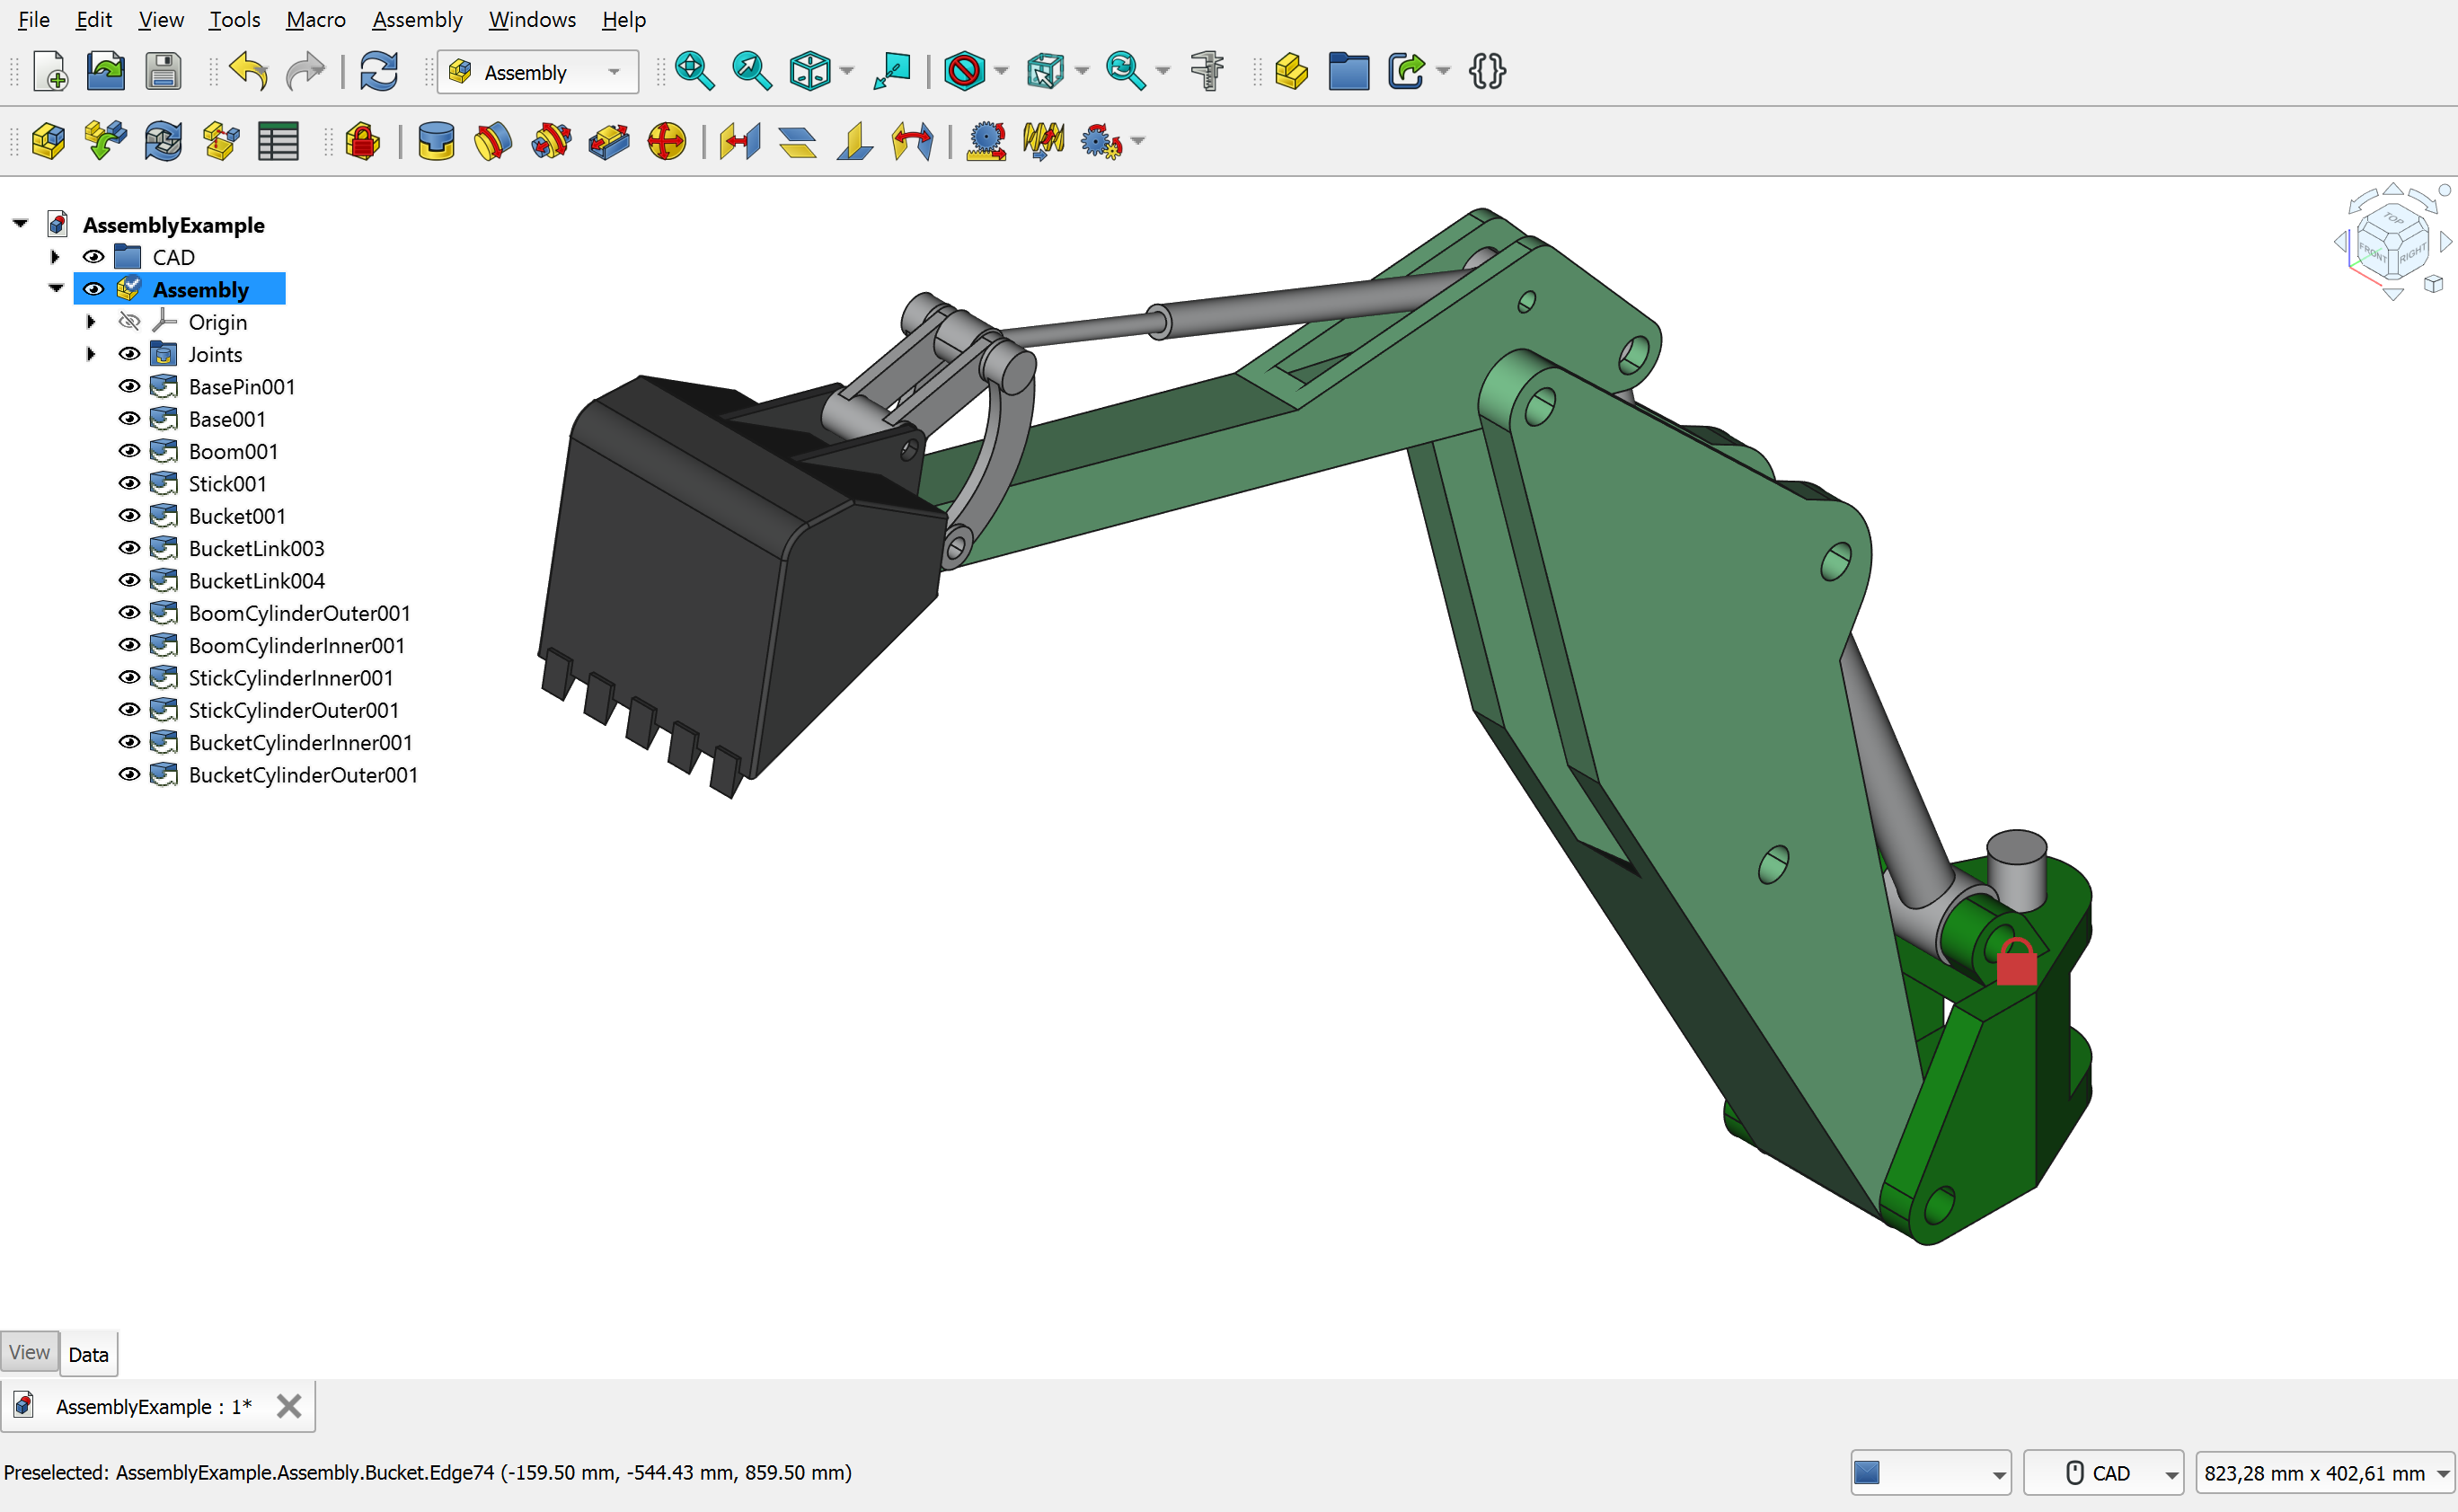
\includegraphics[width=0.8\textwidth]{img/cap11_proyecto.png}
	\caption{Componente mecánico completo diseñado en FreeCAD}
\end{figure}

Proyecto final que integra todos los conocimientos
aprendidos. Diseña un componente mecánico completo
siguiendo estándares de la industria argentina.

%% D. Búsqueda e Inserción de Activos Gráficos
%% Imagen insertada al inicio del capítulo

Proyecto: Soporte para maquinaria agrícola
\begin{itemize}
	\item Sector: Industria agropecuaria argentina
	\item Normas: IRAM y estándares industriales
	\item Requisitos: Resistencia, facilidad de fabricación
\end{itemize}

%% B. Actividades Teóricas
\section{Investigar y responder}
\faPencil

Investiga sobre el proyecto y responde:
\begin{enumerate}
	\item ¿Qué es un soporte mecánico y qué funciones cumple?
	\item ¿Qué materiales se usan comúnmente en soportes
	      agrícolas?
	\item ¿Qué normas argentinas aplican a componentes
	      mecánicos?
	\item ¿Cómo se determinan las cargas que soportará
	      el componente?
	\item ¿Qué procesos de fabricación son comunes en
	      Argentina?
	\item ¿Cómo se asegura la calidad de un componente
	      mecánico?
	\item ¿Qué consideraciones de seguridad deben tenerse?
	\item ¿Cómo se documenta técnicamente un componente
	      industrial?
\end{enumerate}

%% C. Actividades Prácticas
\section{Resolver los siguientes problemas}
\faWrench

Problemas para aplicar conocimientos:
\begin{enumerate}
	\item Diseña el boceto principal del soporte con
	      dimensiones aproximadas.
	\item Aplica restricciones geométricas y dimensionales
	      al boceto.
	\item Crea el sólido principal usando operación de
	      extrusión.
	\item Añade agujeros para tornillería estándar.
	\item Aplica biselados y chaflanados según requerimientos.
	\item Diseña los componentes de sujeción complementarios.
	\item Crea un ensamblaje completo del soporte con
	      tornillería.
	\item Genera planos técnicos con todas las vistas
	      necesarias.
	\item Exporta modelos a STL para posible impresión
	      3D.
	\item Documenta el proyecto completo con especificaciones
	      técnicas y conclusiones.
\end{enumerate}

\section{Evaluación del Proyecto}
\begin{itemize}
	\item Complejidad geométrica: 25 puntos
	\item Uso de restricciones: 20 puntos
	\item Operaciones de modelado: 25 puntos
	\item Planos técnicos: 20 puntos
	\item Documentación: 10 puntos
\end{itemize}

Total: 100 puntos